\begin{figure*}

\begin{minipage}{0.33\linewidth}
  \centering
  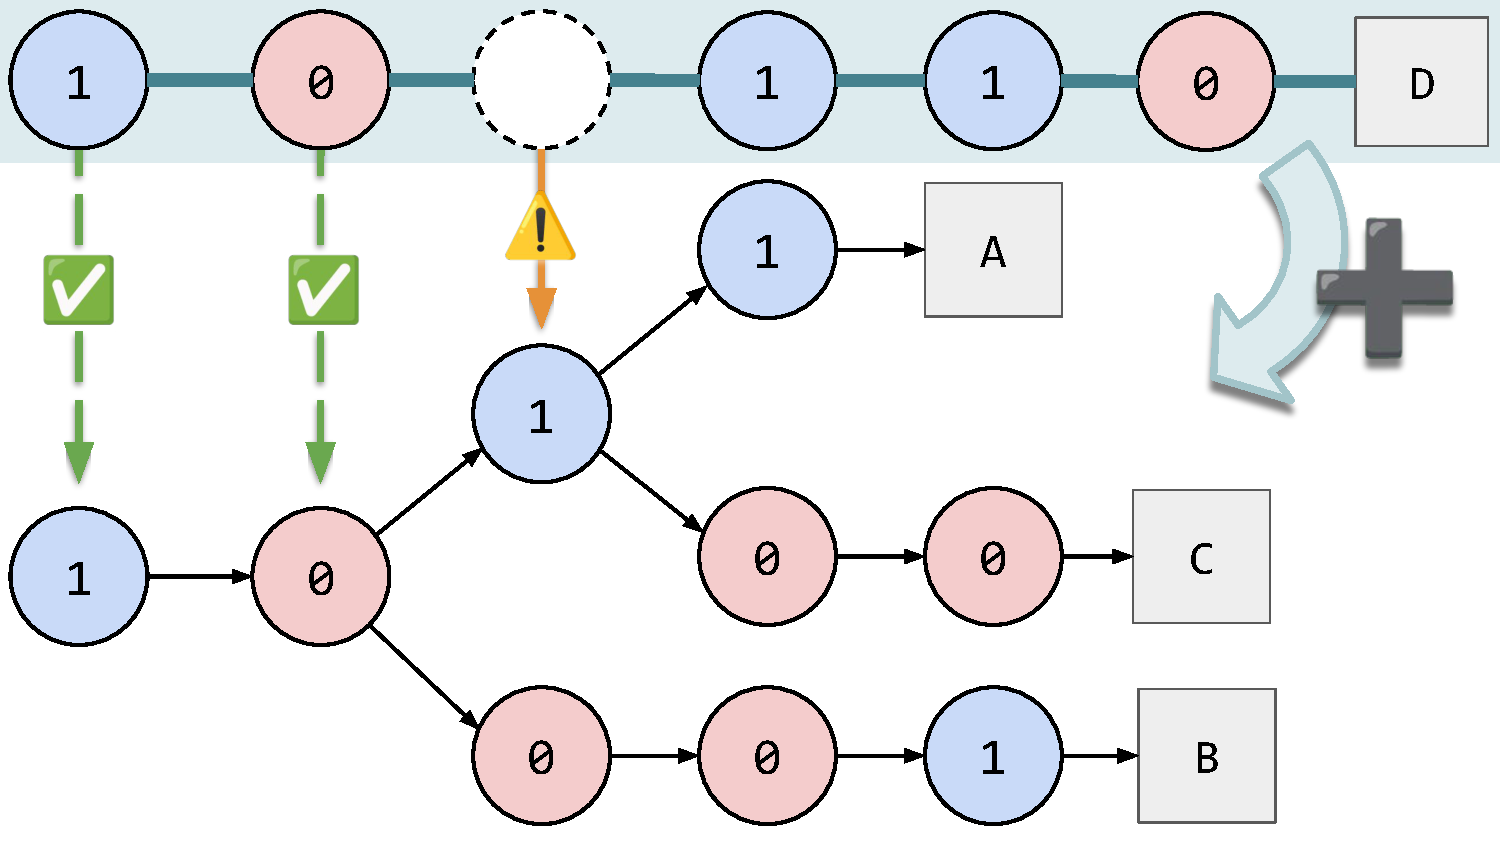
\includegraphics[width=\linewidth]{img/shortcut-algo-diagram-1}
  \subcaption{Preparing to add organism $D$}
  \label{fig:shortcut-algo-diagram-1}
\end{minipage}
\begin{minipage}{0.33\linewidth}
  \centering
  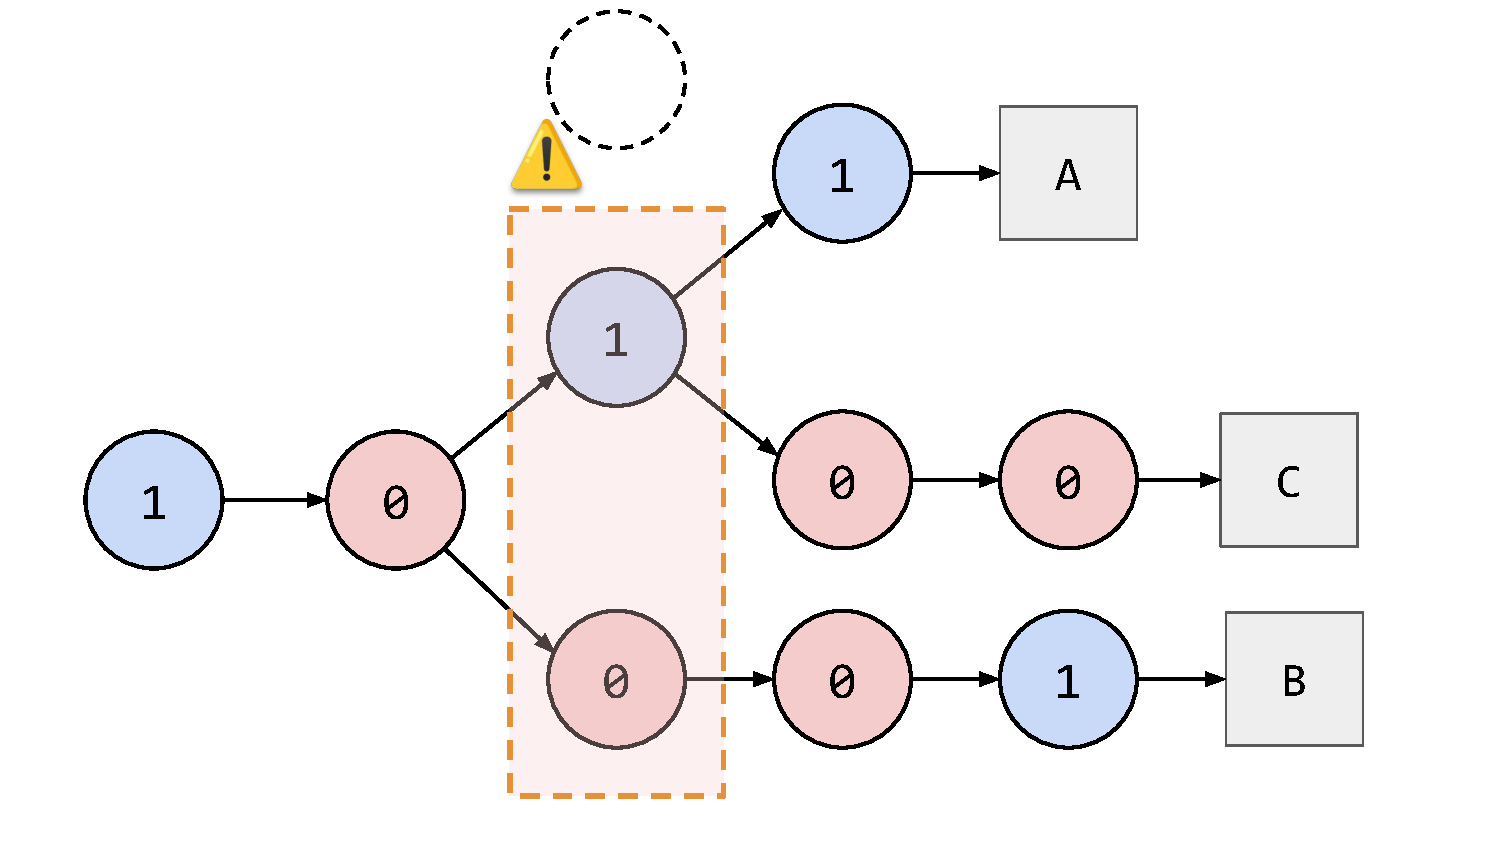
\includegraphics[width=\linewidth]{img/shortcut-algo-diagram-2}
  \subcaption{Encountering dropped marker}
  \label{fig:shortcut-algo-diagram-2}
\end{minipage}
\begin{minipage}{0.33\linewidth}
  \centering
  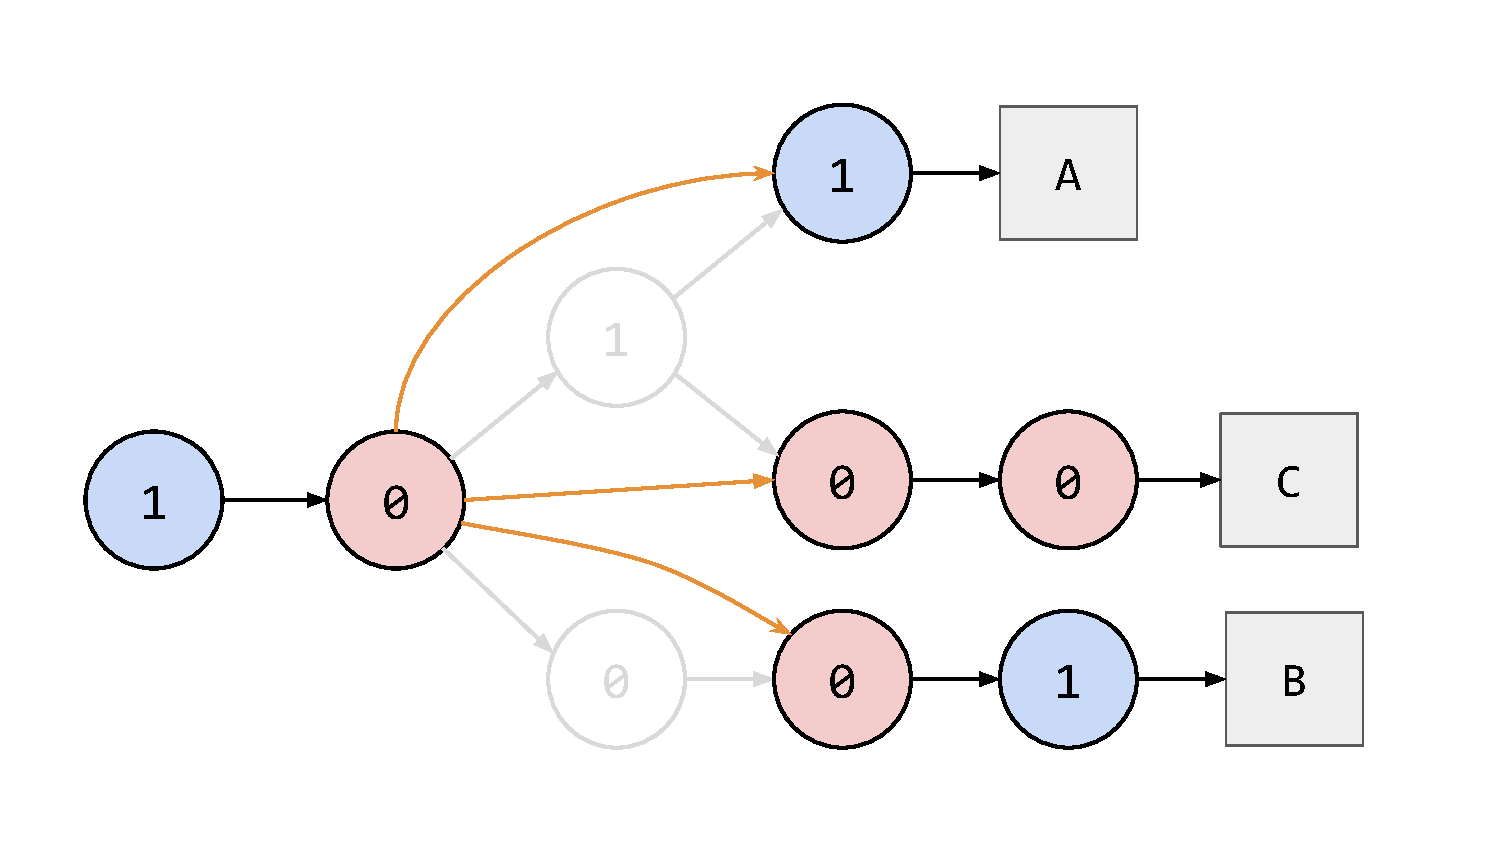
\includegraphics[width=\linewidth]{img/shortcut-algo-diagram-3}
  \subcaption{Shortcuts around dropped-marker nodes}
  \label{fig:shortcut-algo-diagram-3}
\end{minipage}
\begin{minipage}{\linewidth}\par\end{minipage}
\begin{minipage}{0.33\linewidth}
  \centering
  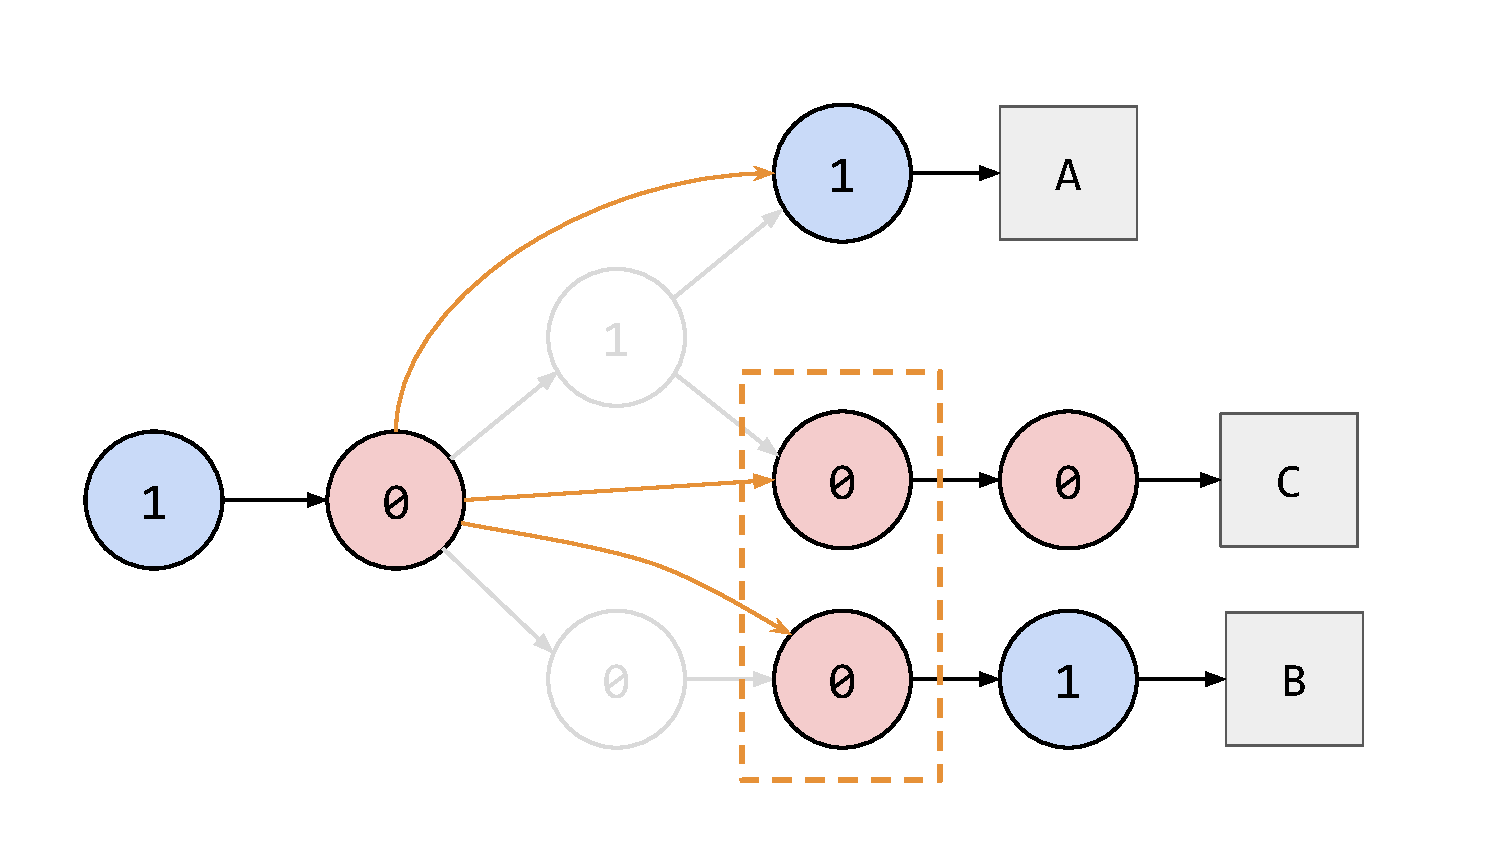
\includegraphics[width=\linewidth]{img/shortcut-algo-diagram-4}
  \subcaption{Encountering redundant shorcuts}
  \label{fig:shortcut-algo-diagram-4}
\end{minipage}
\begin{minipage}{0.33\linewidth}
  \centering
  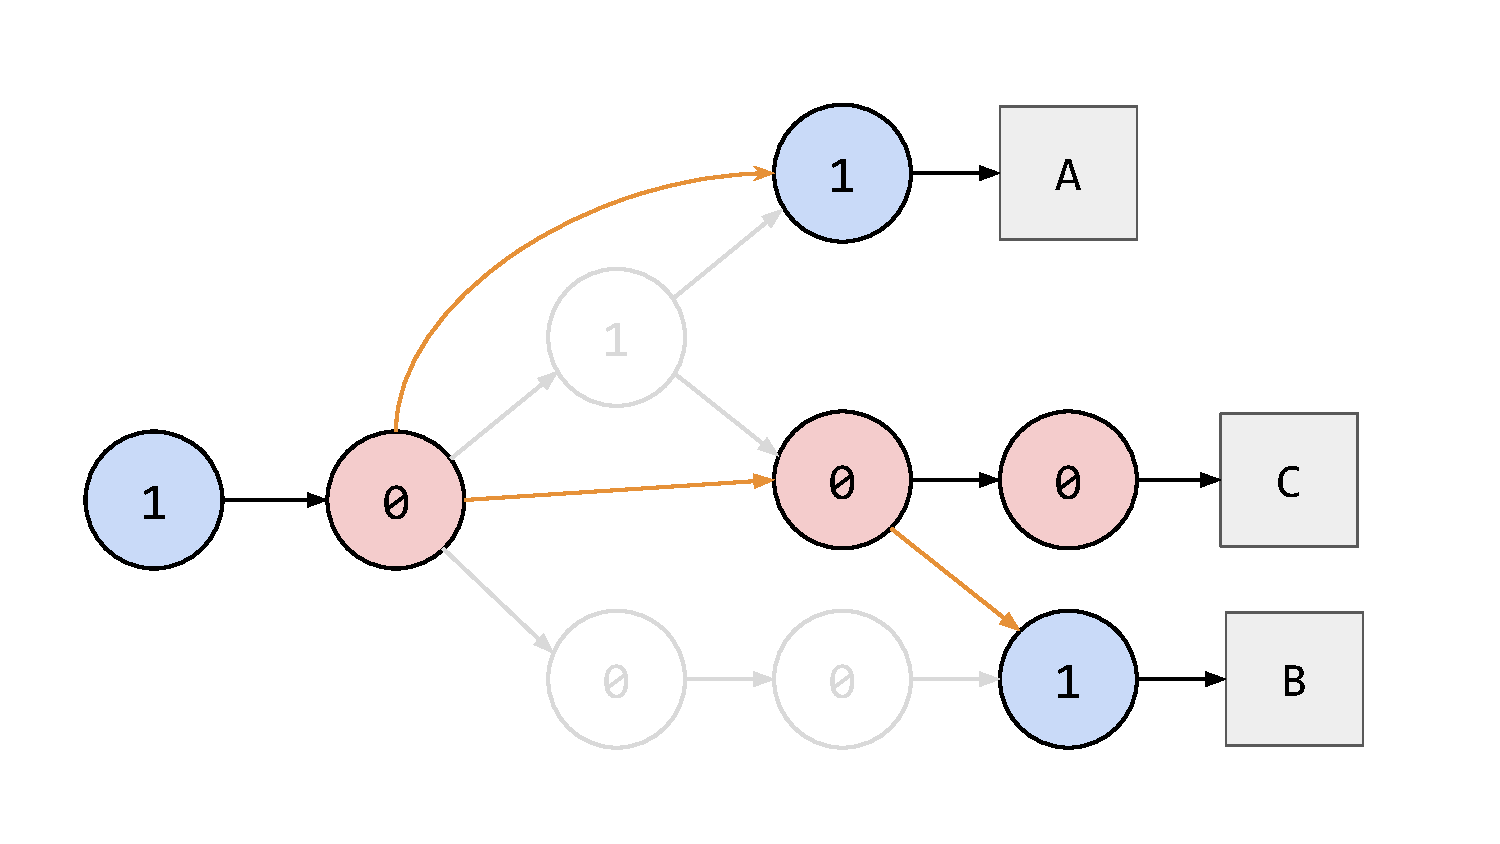
\includegraphics[width=\linewidth]{img/shortcut-algo-diagram-5}
  \subcaption{Collapsing redundant shortcuts}
  \label{fig:shortcut-algo-diagram-5}
\end{minipage}
\begin{minipage}{0.33\linewidth}
  \centering
  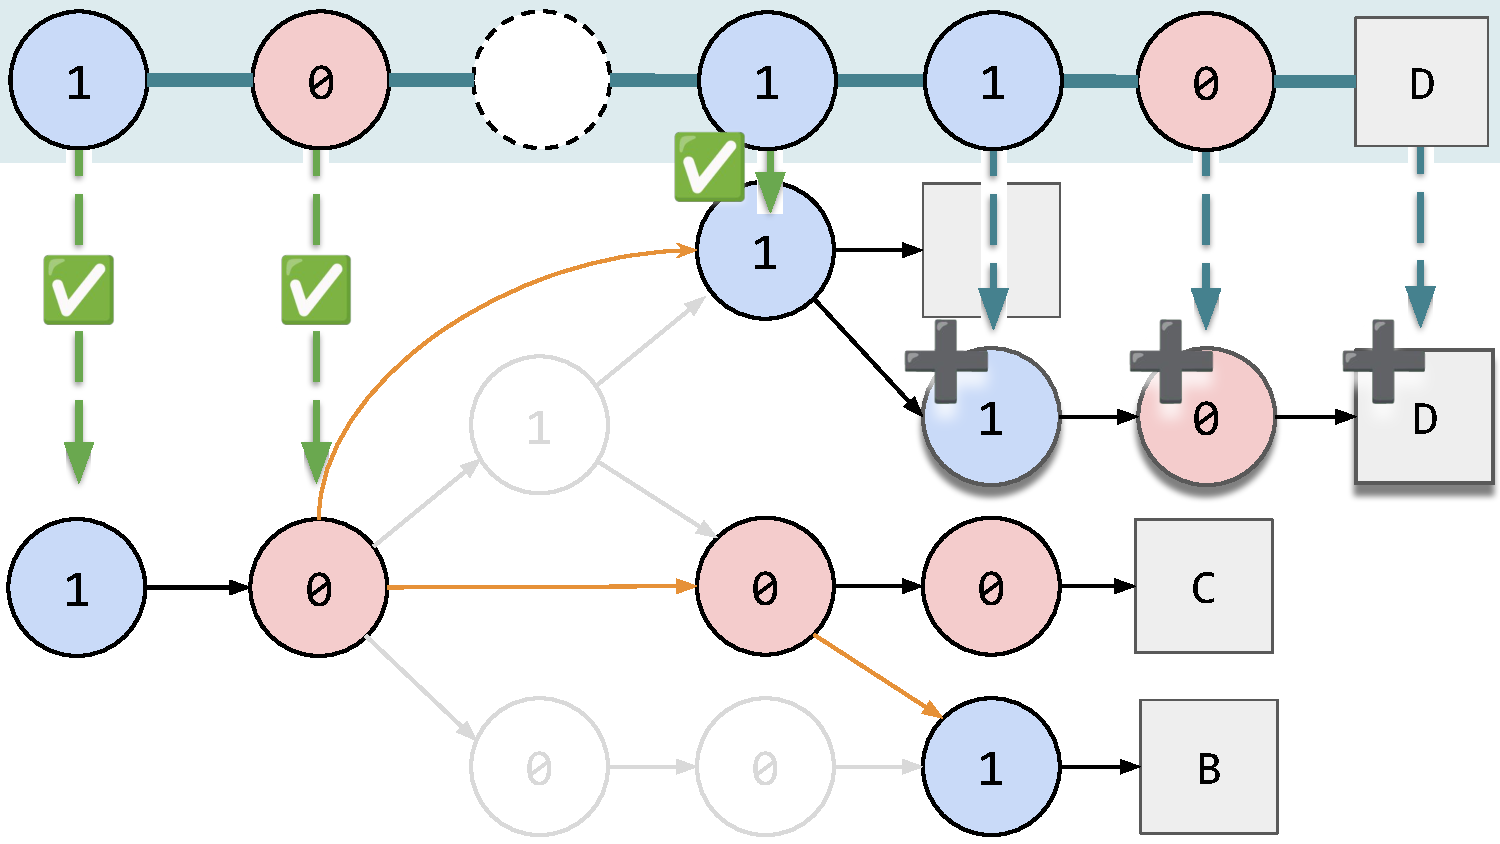
\includegraphics[width=\linewidth]{img/shortcut-algo-diagram-6}
  \subcaption{Organism $D$ added}
  \label{fig:shortcut-algo-diagram-6}
\end{minipage}
\caption{%
\textbf{Trie-consolidation procedure for proposed shortcut algorithm.}
\small
A dropped hereditary marker is encountered while extending trie with genome $D$ (panel \ref{fig:shortcut-algo-diagram-2}).
All subsequent-added genomes will also have dropped markers at this position, so corresponding trie nodes may be bypassed by ``shortcut'' connections (panel \ref{fig:shortcut-algo-diagram-3}).
Note that bypassed trie structure is retained (``grayed-out'' nodes), so corresponding phylogenetic structure remains when reconstruction is finalized.
In a final step, shortcuts leading to identical nodes are further consolidated (panels \ref{fig:shortcut-algo-diagram-4} and \ref{fig:shortcut-algo-diagram-5}).
}
\label{fig:algo-diagram}

\end{figure*}
